\documentclass{article}
\usepackage[utf8]{inputenc}
\usepackage{geometry}
\usepackage{url}
\usepackage[utopia]{mathdesign}
 \geometry{
 a4paper,
 total={170mm,257mm},
 left=20mm,
 top=20mm,
 }
 \usepackage{graphicx}
 \usepackage{titling}

\bibliographystyle{plain}
 \title{The possibility to mimic tentacles of octopuses using soft robotics.
}
\author{GU JUN}
\date{September 30. 2024}
 
 \usepackage{fancyhdr}
\fancypagestyle{plain}{%  the preset of fancyhdr 
    \fancyhf{} % clear all header and footer fields
    \fancyfoot[L]{\thedate}
    \fancyhead[L]{Soft Robotics Home Assignment \#2}
    \fancyhead[R]{\theauthor}
}
\makeatletter
\def\@maketitle{%
  \newpage
  \null
  \vskip 1em%
  \begin{center}%
  \let \footnote \thanks
    {\LARGE \@title \par}%
    \vskip 1em%
    %{\large \@date}%
  \end{center}%
  \par
  \vskip 1em}
\makeatother

\usepackage{lipsum}  
\usepackage{cmbright}

\begin{document}

\maketitle

\noindent\begin{tabular}{@{}ll}
    Student & \theauthor\\
    Student ID & 6132230056-4 \\
\end{tabular}
% working principle, advantage, novelty, and what interests you.

\section*{The features of tentacles}
Tentacles, the limbs of octopuses, could be the most useful executors of all kinds of structures. 
Their power and flexibility can grasp, swim, or even do other tasks. And this is the reason octopuses could be one of the most successful species in the ocean.
However, another feature that interests me more is how these tentacles are controlled, which is the disturbed neutron system\cite{hochner2012embodied}.
In other words, disturbed intelligence is the key that makes tentacles flexible and agile.
This is also a purpose of soft robotics, to achieve a more flexible intelligence.
So my idea is to build a soft robot arm with disturbed intelligence
\begin{figure}[htbp]
  \centering
    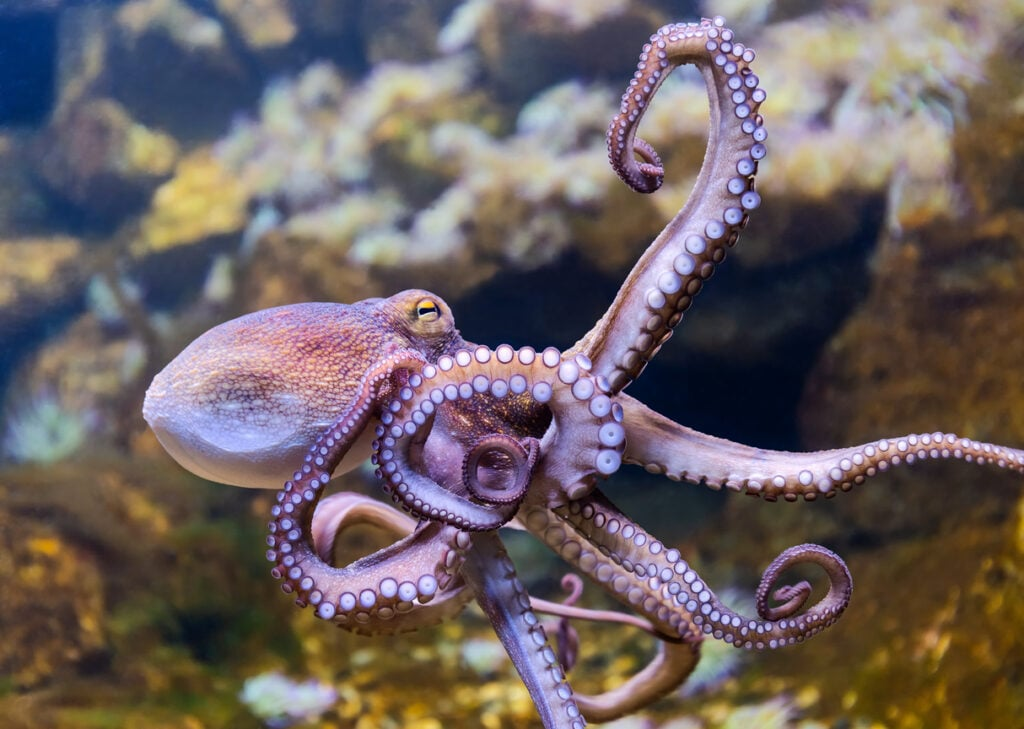
\includegraphics[width=0.2\textwidth]{octopus.jpg}
  \hspace{0.05\textwidth} % Adjust the horizontal space between the figures
    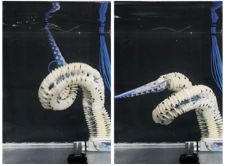
\includegraphics[width=0.2\textwidth]{octupus_robot.png}
  \caption{An octopus and a tentacle-like robot are swinging their arm.}
  \label{fig:side_by_side}
\end{figure}
\section*{What materials, structures, and actuators should be used}
My basic idea is to combine artificial muscles and some flexible electronics.
Tentacles require continuous bending, stretching, and twisting in multiple planes, which artificial muscles can achieve\cite{fras2018bio}.
Although some researchers have tried sensorized tentacles\cite{xie2023octopus}, however, disturbed computation is still a new research area.
We need to make these muscles intelligent to achieve an ideal disturbed motion control system. Flexible electronics\cite{hui2023green} can help here.
However, the most difficult part of this idea would be the algorithm part.
To design a controller that doesn't rely on a centered computation will be necessary.
To make it possible, we may change our perspective to see how motions happen, a new perspective different from traditional kinematics/dynamics.
An algorithm that instead of calculating all things at once, tries to be closer and closer iteratively may be a doable direction.
\section*{Conclusion}
In this report, I present an idea: a soft robot arm prototype inspired by the octopuses. 
Although there are many pieces of research related to octopus-like robots, few mention the interesting disturbed intelligence of the octopuses.
With artificial muscles and flexible electronics, an octopus-inspired embedded controlled robot arm can be achieved.
\bibliography{refs}

\end{document}
